\documentclass[11pt]{article}

\usepackage{latexsym}
\usepackage{graphicx}
\usepackage{amssymb}
\usepackage{amsthm}
\usepackage{enumerate}
\usepackage{amsmath}
\usepackage{cancel}
\numberwithin{equation}{section}

\setlength{\evensidemargin}{.25in}
\setlength{\oddsidemargin}{-.25in}
\setlength{\topmargin}{-.75in}
\setlength{\textwidth}{6.5in}
\setlength{\textheight}{9.5in}
\newcommand{\due}{March 31st, 2011}
\newcommand{\HWnum}{9}
\newcommand{\grad}{\bold\nabla}
\newcommand{\vecE}{\vec{E}}
\newcommand{\scrptR}{\vec{\mathfrak{R}}}
\newcommand{\kapa}{\frac{1}{4\pi\epsilon_0}}
\newcommand{\emf}{\mathcal{E}}
\newcommand{\unit}[1]{\ensuremath{\, \mathrm{#1}}}
\newcommand{\real}{\textnormal{Re}}
\newcommand{\Erf}{\textnormal{Erf}}
\newcommand{\sech}{\textnormal{sech}}
\newcommand{\scrO}{\mathcal{O}}
\newcommand{\levi}{\widetilde{\epsilon}}
\newcommand{\partiald}[2]{\ensuremath{\frac{\partial{#1}}{\partial{#2}}}}
\newcommand{\norm}[2]{\langle{#1}|{#2}\rangle}
\newcommand{\inprod}[2]{\langle{#1}|{#2}\rangle}
\newcommand{\ket}[1]{|{#1}\rangle}
\newcommand{\bra}[1]{\langle{#1}|}





\begin{document}
\begin{titlepage}
\setlength{\topmargin}{1.5in}
\begin{center}
\Huge{Physics 3320} \\
\LARGE{Principles of Electricity and Magnetism II} \\
\Large{Professor Ana Maria Rey} \\[1cm]

\huge{Homework \#\HWnum}\\[0.5cm]

\large{Joe Becker} \\
\large{SID: 810-07-1484} \\
\large{\due} 

\end{center}

\end{titlepage}



\section{Problem \#1}
\begin{enumerate}[(a)]
\item
We know that the kinetic energy of a nearly free electron is given by
\begin{equation}
E = \frac{\hbar^2k^2}{2m}
\label{KinEn}
\end{equation}
where $k^2$ is the magnitude of the wave-vector squared. For a square lattice we have $k^2 = k_x^2+k_y^2$ so equation \ref{KinEn} becomes
$$ E = \frac{\hbar^2}{2m}(k_x^2+k_y^2)$$ 
So if we say that for the wave-vector at a corner of the first zone is given by $(k_x,k_y) = (\pi,\pi)$. We can see that the kinetic energy for this wave-vector is
$$E_{1} = \frac{\hbar^2}{2m}(k_x^2+k_y^2) = \frac{\hbar^2}{2m}(\pi^2+\pi^2) = \frac{\hbar^2\pi^2}{m}$$ 
Now we can see that the midpoint of a side face has the wave-vector $(k_x,k_y) = (\pi,0)$. Note that the first Brillouin zone goes from $-\pi$ to $\pi$ this implies that the midpoint is $0$. So the kinetic energy at this point is
$$E_{2} = \frac{\hbar^2}{2m}(\pi^2+(0)^2) = \frac{\hbar^2\pi^2}{2m}$$ 
Now it is easy to see that the ratio of the two kinetic energies is
\begin{align*}
\frac{E_1}{E_2} &= \frac{\hbar^2\pi^2}{m}\frac{2m}{\hbar^2\pi^2} = 2
\end{align*}
So the kinetic energy at the corner is greater than the kinetic energy at the midpoint of a side by a factor of 2.


\item
It is easy to see for a simple cubic lattice we add an extra dimension so the wave-vector at the corner of the first Brillouin zone is $(k_x,k_y,k_z) = (\pi,\pi,\pi)$ and at the center of a face we have the wave-vector $(k_x,k_y,k_z) = (\pi,0,0)$. These wave vectors and equation \ref{KinEn} implies that 
$$E_1 = \frac{3\hbar^2\pi^2}{2m}$$
and
$$E_2 = \frac{\hbar^2\pi^2}{2m}$$
So the kinetic energy at the corner of the first zone is a factor of 3 greater that the kinetic energy at the center of a face.

\item
The result from part (b) implies that the there is a large amount of energy to get to the corner of the first Brillouin zone so the valence electrons will jump the gap and fill the band in the second Brillouin zone rather than filling the entire band in the first zone.
\end{enumerate}

\section{Problem \#2}
We know that the energy of a free particle is given by equation \ref{KinEn}
$$E = \frac{\hbar^2k^2}{2m}$$
and that for the face-centered cubic lattice the primitive basis vectors are given by
\begin{align*}
\vec{b}_1 &= \frac{2\pi}{a}(-\hat{x}+\hat{y}+\hat{z})\\
\vec{b}_2 &= \frac{2\pi}{a}(\hat{x}-\hat{y}+\hat{z})\\
\vec{b}_3 &= \frac{2\pi}{a}(\hat{x}+\hat{y}-\hat{z})
\end{align*}
So for the energy bands outside the first Brillouin zone we need to subtract or add a reciprocal lattice vector $\vec{G}$ which is given by
\begin{align*}
\vec{G} &= h\vec{b}_1 + k\vec{b}_2 + l\vec{b}_3\\
&= \frac{2\pi}{a}\left(\frac{}{}h(-\hat{x}+\hat{y}+\hat{z}) + k(\hat{x}-\hat{y}+\hat{z}) + l(\hat{x}+\hat{y}-\hat{z})\right)\\
&= \frac{2\pi}{a}\left(\frac{}{}(-h+k+l)\hat{x} + (h-k+l)\hat{y} + (h+k-l)\hat{z}\right)
\end{align*}
where $h,k$, and $l$ are integers. Now we want to find all the energy bands that have energy that is less than six times the lowest band energy at the zone boundary at 
$$\vec{k} = \frac{2\pi}{a}\left(\frac{1}{2},\frac{1}{2},\frac{1}{2}\right)$$
Note for simplicity we will take $\hbar^2/2m =1$ so the energy at the zone boundary by equation \ref{KinEn} is
\begin{align*}
E &= \cancelto{1}{\frac{\hbar^2}{2m}}k^2\\
&= \left(\frac{2\pi}{a}\right)^2\left[\left(\frac{1}{2}\right)^2+\left(\frac{1}{2}\right)^2+\left(\frac{1}{2}\right)^2\right]\\
&= \frac{3}{4}\left(\frac{2\pi}{a}\right)^2
\end{align*}
So we want to find all the $h,k,l$ such that the energy is less than 
$$E = \frac{9}{2}\left(\frac{2\pi}{a}\right)^2$$
where the energy is given by
$$E = (\vec{k} - \vec{G})^2$$
note that the $\vec{G}$ determines the zero of the parabola in $k$-space. We already found the lowest energy for $(h,k,l) = (0,0,0)$. We can find the energy for any $(h,k,l)$ as
\begin{align*}
E &= (\vec{k} - \vec{G})^2\\
&= \left(\frac{2\pi}{a}\right)^2\left[\left(h-k-l\right)^2 +\left(-h+k-l\right)^2 +\left(-h-k+l\right)^2\right]
\end{align*}
Note that the factor of with the $2\pi$ will be neglected for simplicity as it is consistent with every term. So the calculated energies are given in table \ref{TabProb2}
\begin{table}
\begin{centering}
\begin{tabular}{cc}
$(hkl)$	&Energy ($E(hkl)$)\\
\hline
$(100)$	&$3$ \\
$(010)$	&$3$ \\
$(001)$	&$3$ \\
$(111)$	&$3$ \\
$(\overline{1}00)$	&$3$ \\
$(0\overline{1}0)$	&$3$ \\
$(00\overline{1})$	&$3$ \\
$(\overline{111})$	&$3$ \\
$(110)$	&$4$ \\
$(101)$	&$4$ \\
$(011)$	&$4$ \\
$(\overline{1}\overline{1}0)$	&$4$ \\
$(\overline{1}0\overline{1})$	&$4$ \\
$(0\overline{1}\overline{1})$	&$4$ \\
\end{tabular}
\caption{\it{The energies for the reciprocal lattice vectors up to six times the lowest energy band. Note we neglect the factor of $(2\pi/a)^2$.}}
\label{TabProb2}
\end{centering}
\end{table}
So we plotted the bands for each of these reciprocal lattice vectors in figure \ref{Plot1}. Note the zero is the distance between the node that $\vec{G}$ points to from the edge of the Brillouin zone. 
\begin{figure}[h]
\centering
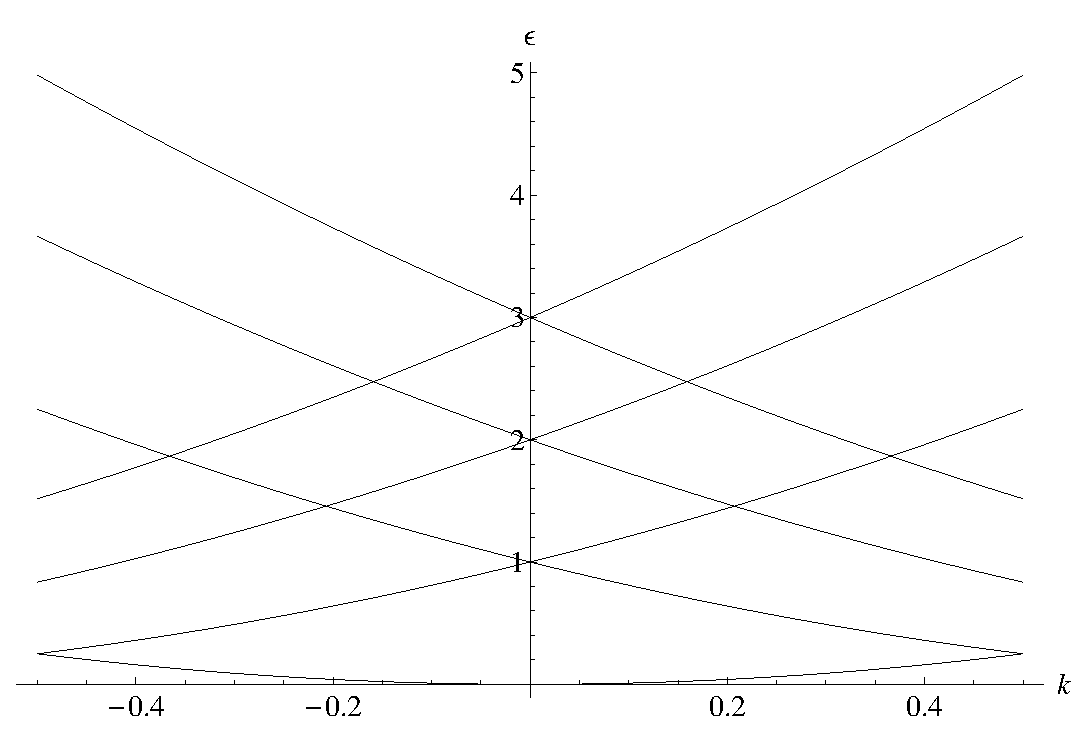
\includegraphics[scale=0.55]{Plot1.eps}
\caption{\it{Plot of the energy bands}}
\label{Plot1}
\end{figure}

\section{Problem \#3}
For a square lattice in two dimensions we are given the crystal potential as
$$U(x,y) = -4U\cos(2\pi x/a)\cos(2\pi y/a)$$
we can apply the central equation 
\begin{equation}
(\lambda_k - \epsilon)C(k) +\sum_{G}U_GC(k-G) = 0
\label{central}
\end{equation}
where
$$\lambda_k = \frac{\hbar^2k^2}{2m}$$
We see that $U(x,y)$ contains the lattice vectors $(\pm 1,\pm1)$ so we can say that equation \ref{central} becomes the system
\begin{align*}
(\lambda_k - \epsilon)C(1,1) +\sum_{G}U_GC(-1,-1) &= 0\\
(\lambda_k - \epsilon)C(-1,-1) +\sum_{G}U_GC(1,1) &= 0
\end{align*}
This implies that the gap spacing is $2U$. Where $U$ is given in $U(x,y)$




\end{document}

